\documentclass[border=3pt]{standalone}
% Preâmbulo compartilhado pelos diagramas TikZ da aula 8 de IHC (Design de IHC)
\usepackage[T1]{fontenc}
\usepackage[utf8]{inputenc}
\usepackage{lmodern}
\usepackage{amsmath}
\usepackage{xcolor}
\usepackage{tikz}
\usetikzlibrary{arrows.meta,angles,quotes,decorations.pathmorphing,decorations.pathreplacing,calc,
                positioning,shapes.geometric,shapes.misc,backgrounds,fit,
                math}

% Paleta (mesma dos SVGs originais)
% Paleta da disciplina de IHC: acento roxo (#755099), da capa do livro.
% (o nome "dblue" é mantido para não alterar todos os diagramas)
\definecolor{dblue}{HTML}{755099}
\definecolor{dorange}{HTML}{B3541E}
\definecolor{dgreen}{HTML}{4A7C59}
\definecolor{dred}{HTML}{9C4B4B}
\definecolor{dcream}{HTML}{F4F1EA}
\definecolor{dshade}{HTML}{DDD7C9}

% Função gaussiana (não normalizada por padrão de escala visual)
\pgfmathdeclarefunction{gauss}{3}{%
  \pgfmathparse{1/(#3*sqrt(2*pi))*exp(-((#1-#2)^2)/(2*#3^2))}%
}

% Estilos comuns (prefixo d... para não colidir com chaves internas do pgf)
\tikzset{
  >={Stealth[length=2mm]},
  dguide/.style={gray!55, dashed, line width=0.4pt},
  daxis/.style={gray!60, line width=0.7pt, ->},
  dbody/.style={fill=black!3, draw=black!80, line width=1pt},
  dacc/.style={draw=dblue, line width=1pt},
  dlbl/.style={black!55, font=\small},
  dsub/.style={black!45, font=\footnotesize},
  dstate/.style={circle, draw=black!80, fill=dcream, line width=1pt,
                 minimum size=17mm, font=\large, inner sep=1pt},
  dobs/.style={circle, draw=black!80, fill=dshade, line width=1pt,
               minimum size=14mm, font=\large, inner sep=1pt},
  dbox/.style={rounded corners=2pt, draw=black!80, fill=dcream, line width=1pt,
               align=center, inner sep=6pt},
  dop/.style={circle, draw=black!80, fill=white, line width=1pt,
              minimum size=6mm, inner sep=0pt, font=\small},
  dtrans/.style={->, dblue, line width=1pt},
  dmeas/.style={->, dorange, line width=1pt},
  dcurve/.style={line width=1pt, dblue},
  dcurveb/.style={line width=1.4pt, dorange},
}

\begin{document}
\hyphenpenalty=10000 \exhyphenpenalty=10000 \tolerance=9999 \emergencystretch=3em
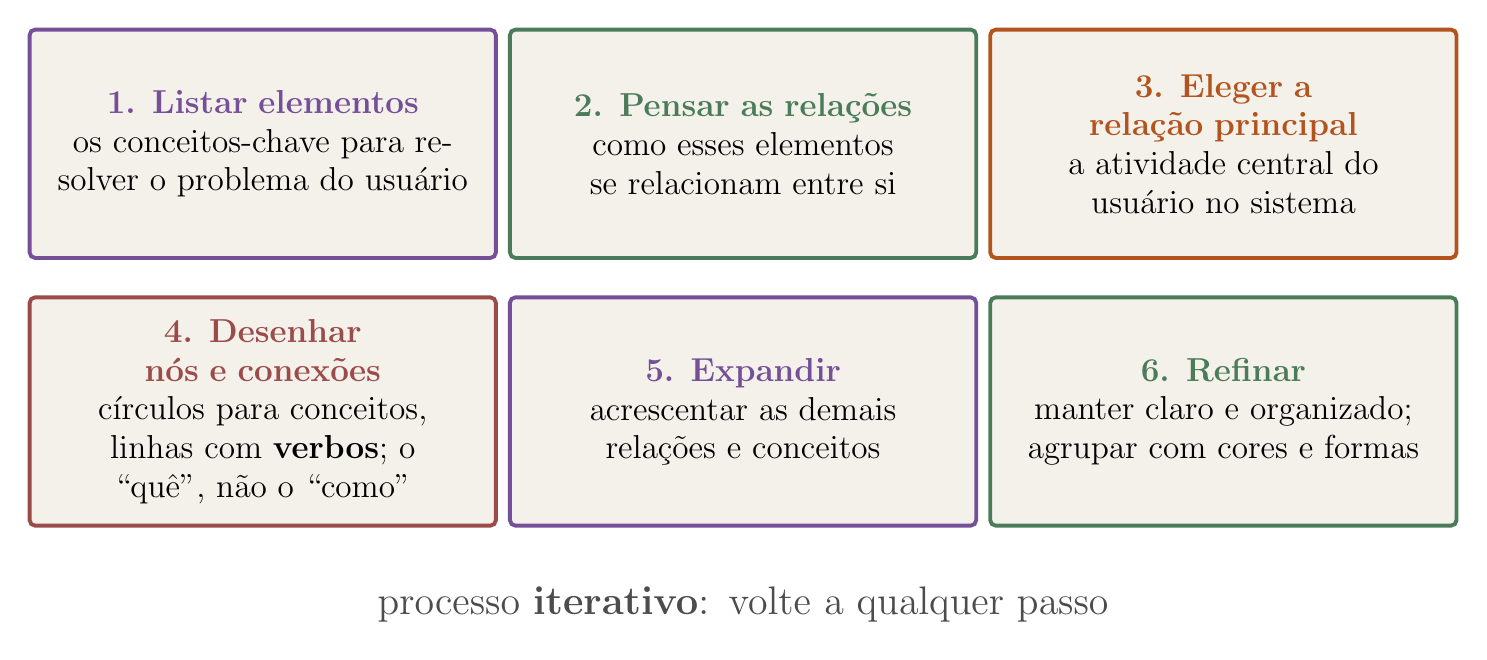
\begin{tikzpicture}[x=1cm,y=1cm]
\tikzset{c/.style={dbox, text width=5.5cm, minimum height=2.9cm, font=\large, line width=1.4pt}}
\node[c, draw=dblue] at (0.0,0.0) {\textbf{\textcolor{dblue}{1. Listar elementos}}\\ os conceitos-chave para resolver o problema do usuário};
\node[c, draw=dgreen] at (6.1,0.0) {\textbf{\textcolor{dgreen}{2. Pensar as relações}}\\ como esses elementos se relacionam entre si};
\node[c, draw=dorange] at (12.2,0.0) {\textbf{\textcolor{dorange}{3. Eleger a relação principal}}\\ a atividade central do usuário no sistema};
\node[c, draw=dred] at (0.0,-3.4) {\textbf{\textcolor{dred}{4. Desenhar nós e conexões}}\\ círculos para conceitos, linhas com \textbf{verbos}; o ``quê'', não o ``como''};
\node[c, draw=dblue] at (6.1,-3.4) {\textbf{\textcolor{dblue}{5. Expandir}}\\ acrescentar as demais relações e conceitos};
\node[c, draw=dgreen] at (12.2,-3.4) {\textbf{\textcolor{dgreen}{6. Refinar}}\\ manter claro e organizado; agrupar com cores e formas};
\node[font=\Large, black!70, text width=17cm, align=center] at (6.1,-5.85) {processo \textbf{iterativo}: volte a qualquer passo};
\end{tikzpicture}
\end{document}
